\hypertarget{cap2}{}
\chapter{Resultados}

Os parâmetros que utilizaremos nas simulações estão listados na tabela
\ref{tabela}.
\begin{table}[!htb]
	\begin{minipage}[b]{0.49\linewidth}
	  \begin{center}
	    \begin{tabular}{c l l}
	\multicolumn{3}{l}{MBBA} \\ 
	\hline 
	\hline 
	$a$               & $= \, 0,0867 \times 10^{6}$   & ${\rm J/Km}^{3}$ \\
	$B$               & $= \, -2,12  \times 10^{6}$   & ${\rm J/m}^{3}$  \\
	$C$               & $= \, 1,74   \times 10^{6}$   & ${\rm J/m}^{3}$  \\
	$\mathcal{L}1$    & $= \, 6,93   \times 10^{-12}$ & ${\rm N}$        \\
	$\mathcal{L}2$    & $= \, 0,0    \times 10^{-12}$ & ${\rm N}$        \\
	$(T-T^{*})$       & $= \, (307,0- 311,0)$         & ${\rm K}$        \\
	$\Delta$          & $= \, 1,0    \times 10^{-9}$  & ${\rm m}$        \\
	$\Delta t$        & $= \, 3,5    \times 10^{-9}$  & ${\rm s}$        \\
	$\mu_1$           & $= \, 0,2 $                   & ${\rm Pa\, s}$   \\
	$\Delta \epsilon$ & $= \, -0,6$                   &                  \\
	$S_{\rm eq}$      & $= \, 0,62$                   &                  \\
	\hline
	    \end{tabular}
	  \end{center}
	\end{minipage}
	\begin{minipage}[b]{0.49\linewidth}
	  \begin{center}
	    \begin{tabular}{c l l}
	\multicolumn{3}{l}{5CB} \\ 
	\hline
	\hline 
	$a$               & $= \, 0,14  \times 10^{6}$   & ${\rm J/Km}^{3}$ \\
	$B$               & $= \, -1,80 \times 10^{6}$   & ${\rm J/m}^{3}$  \\
	$C$               & $= \, 3,60  \times 10^{6}$   & ${\rm J/m}^{3}$  \\
	$\mathcal{L}1$    & $= \, 3,0   \times 10^{-12}$ & ${\rm N}$        \\
	$\mathcal{L}2$    & $= \, 0,0   \times 10^{-12}$ & ${\rm N}$        \\
	$(T-T^{*})$       & $= \, (298,0- 307,2)$        & ${\rm K}$        \\
	$\Delta$          & $= \, 1,0   \times 10^{-9}$  & ${\rm m}$        \\
	$\Delta t$        & $= \, 15    \times 10^{-9}$  & ${\rm s}$        \\
	$\mu_1$           & $= \, 0,3 $                  & ${\rm Pa\, s}$   \\
	$\Delta \epsilon$ & $= \, 11,5$                  &                  \\
	$S_{\rm eq}$      & $= \, 0,58$                  &                  \\
	\hline
	    \end{tabular}
	  \end{center}
	\end{minipage}
	\caption{{\small Parâmetros dos cristais líquidos
MBBA (4-methoxybenzylidene-4-butylanaline) e 5CB
(4-cyano-4'-pentylbiphenyl).}}
	\label{tabela}
\end{table}

A tabela \ref{tabela1} mostra como destacar algumas partes da tabela.
\begin{table}[!htb]
  \begin{center}
    \begin{tabular}{ l | c | c | c }
& $\Delta =0,9 {\rm nm}$ & $\Delta =1,0 {\rm nm}$ & $\Delta =1,5 {\rm
nm}$ \\
		\hline
$\Gamma =1$ & $0,409\pm 0,004$ & \cellcolor[gray]{0.9} $0,412\pm 0,004$
& $0,409\pm 0,009$ \\
		\hline
$\Gamma =\frac{1}{(1-{\rm Tr}{\bf Q}^2)^2}$ & \cellcolor[gray]{0.9}
$0,413\pm 0,004$ & $0,409\pm 0,002$ & $0,406\pm 0,009$ \\
		\hline
    \end{tabular}
  \end{center}
\caption{Comparação entre os expoentes $\alpha$ obtidos pelo
ajuste dos dados de uma média de $100$ condições iniciais de uma rede
de $256 \times 256$ utilizando a lei de potências, $L(t) \varpropto
t^{\alpha}$.}
	\label{tabela1}
\end{table}

Veja as figuras \ref{figura-1} e \ref{figura-2}. Também observe a figura
\ref{MBBA-3}.

\begin{figure}[!htb]
  \centering
		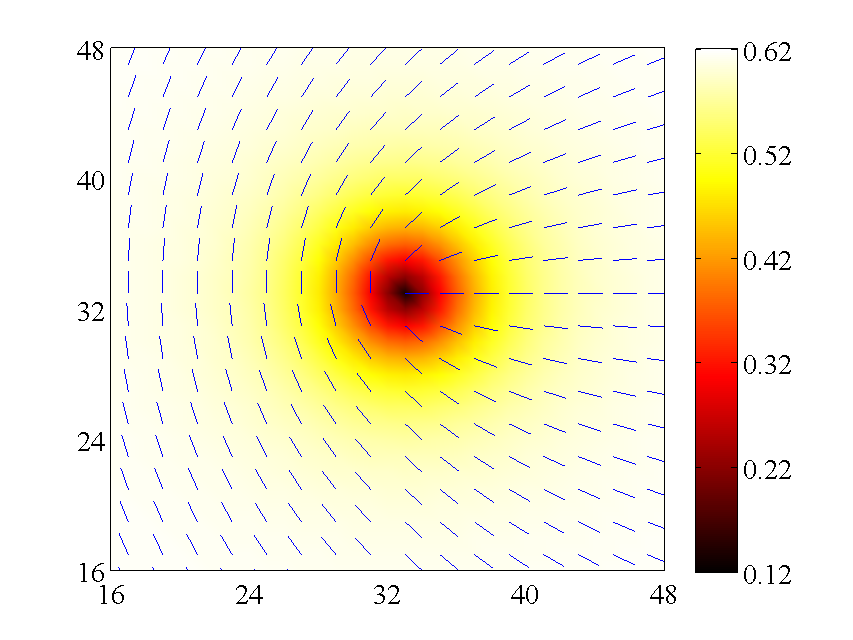
\includegraphics[width= 7.0cm]{fig/fig-1}
  \caption{A figura mostra o perfil de $S$ junto com a projeção do
diretor no plano $x-y$}
  \label{figura-1}
\end{figure}

\begin{figure}[!htb]
  \centering
		\subfloat[$t= 0$  ]{\label{MBBA-1}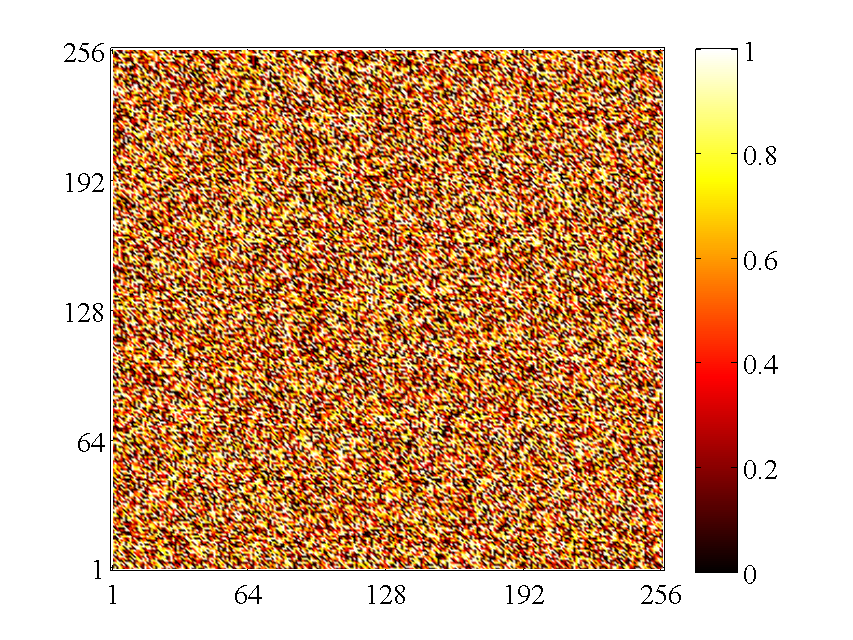
\includegraphics[scale= 0.55]{fig/MBBA-1}}
		\subfloat[$t= 2$  ]{\label{MBBA-2}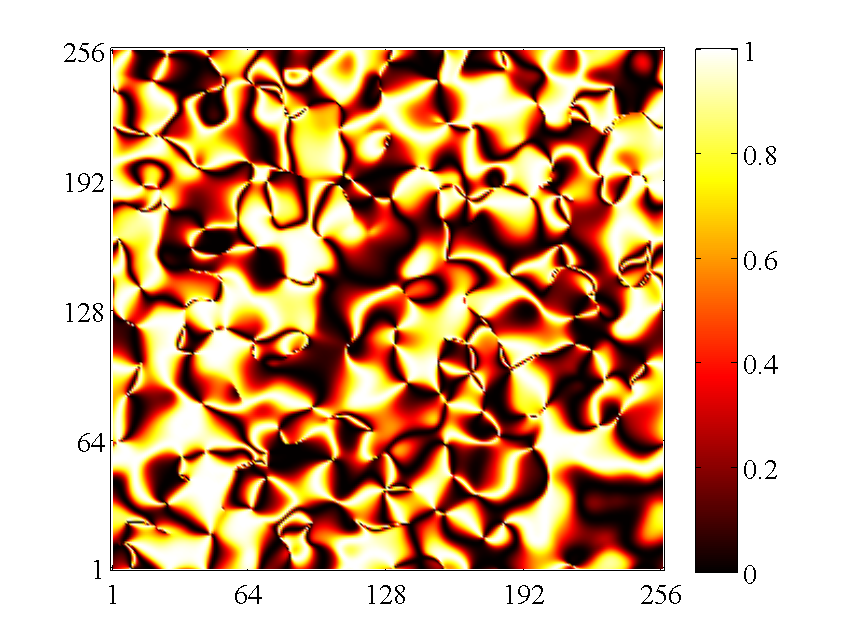
\includegraphics[scale= 0.55]{fig/MBBA-2}}
		\\
		\subfloat[$t= 20$ ]{\label{MBBA-3}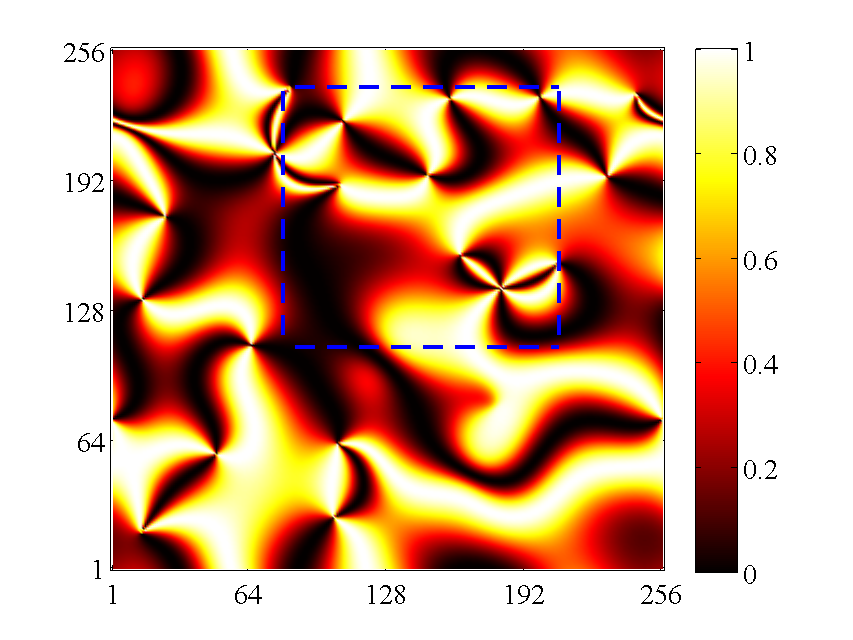
\includegraphics[scale= 0.55]{fig/MBBA-3}}
		\subfloat[$t= 200$]{\label{MBBA-4}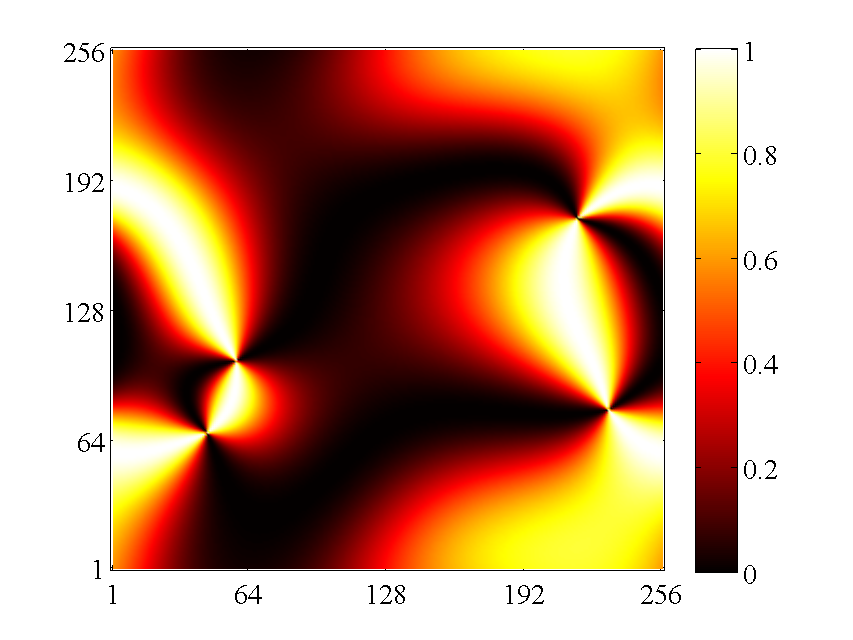
\includegraphics[scale= 0.55]{fig/MBBA-4}}
  \caption{Nesta sequência temporal de imagens é mostrado o valor
do ${\rm sen}^2(2\beta)$ em cada ponto da rede, onde $\beta$ é o ângulo
que o diretor forma com o eixo do polarizador que, neste caso, coincide
com o eixo horizontal.}
  \label{figura-2}
\end{figure}
